%!TEX root = ../../root.tex

\emph{Early stopping} is a regularization technique that stops training as soon as performance on a validation set decreases.

\paragraph{U-shaped curve}
When training large models with sufficient representational capacity to overfit
the task, we often observe that training error decreases steadily over time, but
\emph{validation error} begins to rise again.
\begin{figure}[H]
    \centering
    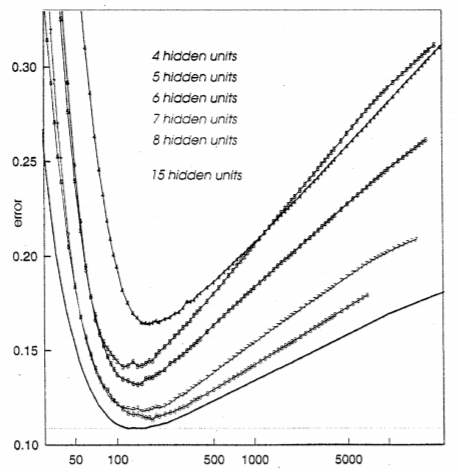
\includegraphics[width=.3\textwidth]{09/7_27}
    \caption{Plot of the validation error when increasing the training time showing a typical U-shape. Each curve corresponds to a different model size (increasing from top to bottom).}	
\end{figure}
A U-shape plot shows how as the training goes on, the validation error decreases and then increases again, while the training error always decreases: when this happens it means that the model is overfitting on the training data.
The plot suggests that there exists a moment in time at which the training should stop, because from that point on the validation error would increase, so the model is not getting better at the (general) task, but is in fact getting worse. 

Things to keep in mind:
\begin{itemize}
    \item Small networks can also overfit.
    \item Large networks have best performance \emph{if they stop early}.
\end{itemize}

However, there is no fixed recipe.
\begin{itemize}
    \item Different models, with different loss functions, on different tasks, with different datasets, would exhibit different curves. From now assume to use \emph{SGD} to train a \emph{MLP}.
    \item Since we have to take decision on whether to stop or not ``on the fly'', we cannot be certain that at the current moment the validation loss is definitely increasing, but might be just a temporary increase due to noise. For this reason it is useful in practice to define \emph{patience} as the numers of training steps (or epochs) we allow the validation loss to increase. If after such interval of time the validation loss has not decreased by at least some amount $\Delta \ell$, we assert that it is indeed definitely increasing.
\end{itemize}

% The underlying idea behind early stopping is that one could see a large network as a superposition of many small networks.
% \begin{center}
%     Large network $\approx$ superposition of small networks.
% \end{center} 
% The intuition is telling us that at the beginning of training, the large network
% is behaving similarly to a small network and as the training goes on the large network stats to capture more and more complex phenomenon. Increasing the training time is like superposing more networks to generate the final, large network. However this modelling of a large net as many small nets depends on the optimization algorithm.
% (e.g. for some optimization algorithm the U-shape validation error behaviour may not take place).
% From now assume to use \emph{Stochastic Gradient Descent}.

% \begin{minipage}{\textwidth}

\paragraph{Overfitting}

It is important to note that it is not always true that more parameters lead to overfitting.
\begin{figure}[H]
    \centering
    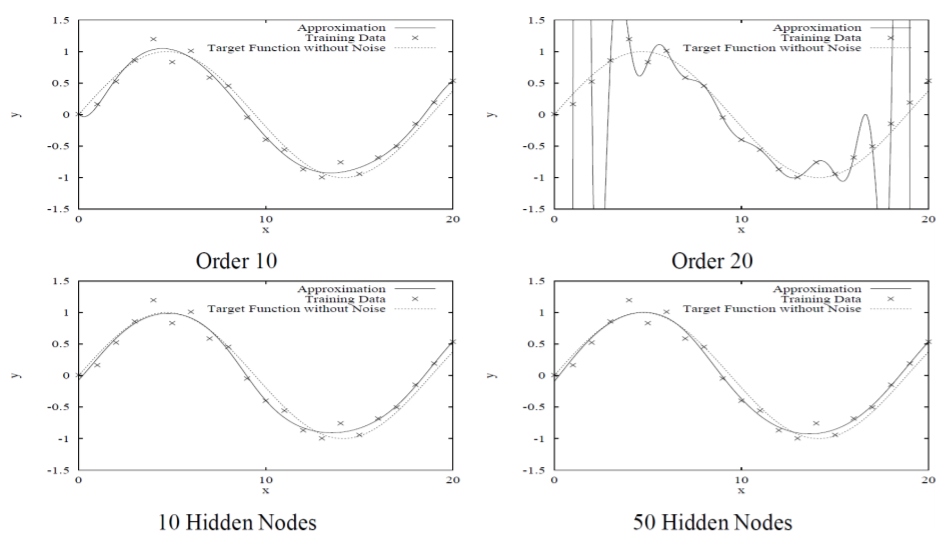
\includegraphics[width=.9\textwidth]{09/9_27}
    \caption{More MLP parameters \emph{not} leading to overfitting.}	
\end{figure}

\begin{figure}[H]
    \centering
    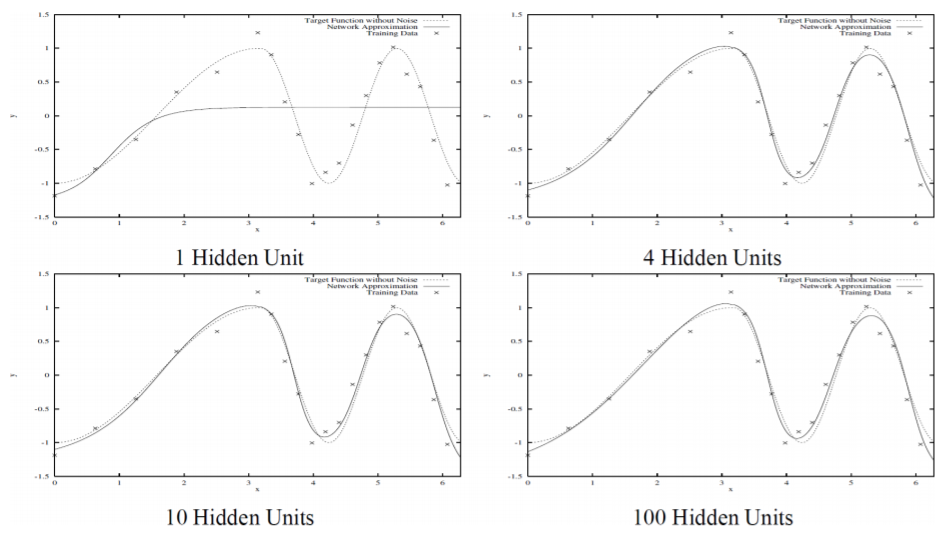
\includegraphics[width=.9\textwidth]{09/10_27}
    \caption{Good fit over all the different \emph{data regions}.}	
\end{figure}
% \end{minipage}

% \begin{minipage}{\textwidth}
Overfitting is \emph{local} and can vary significantly in different regions:
\begin{figure}[H]
    \centering
    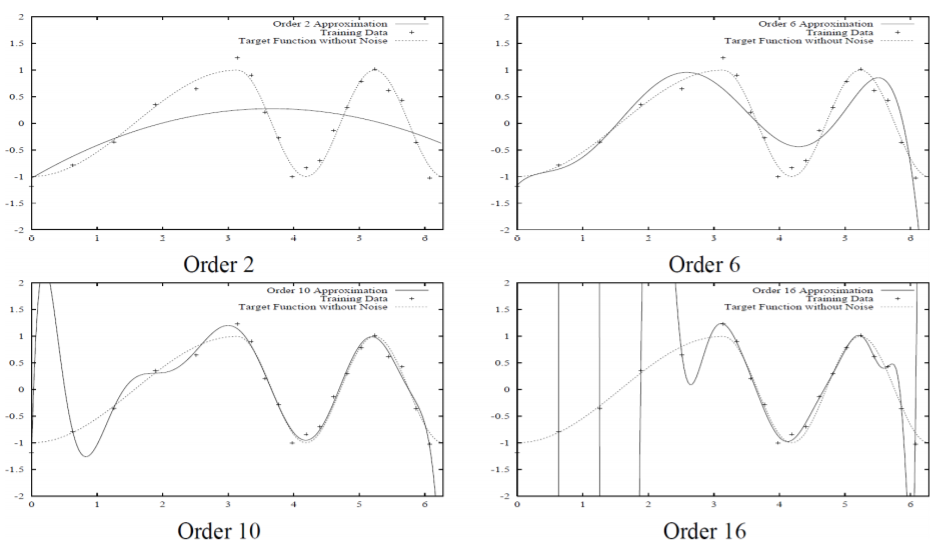
\includegraphics[width=.9\textwidth]{09/11_27}
    \caption{Example of overfitting and underfitting in localized \emph{data regions}.}	
\end{figure}

\begin{figure}[H]
    \centering
    \begin{subfigure}[t]{0.45\textwidth}
        \centering
        \begin{overpic}[width=.5\linewidth]{09/underfitting_high_nonlinearity}\end{overpic}
        \caption{Avoid underfitting regions of \emph{high} nonlinearity.}
    \end{subfigure}
    \hfill
    \begin{subfigure}[t]{0.45\textwidth}
        \centering
        \begin{overpic}[width=.5\linewidth]{09/overfitting_low_nonlinearity}\end{overpic}
        \caption{Avoid overfitting regions of \emph{low} nonlinearity.}
    \end{subfigure}
    \caption{Two important requirements for \emph{early stopping}.}
\end{figure}
% \end{minipage}

\paragraph{Double descent (Capacity-wise double U-shape)}

% \begin{figure}[H]
%     \centering
%     \begin{subfigure}[t]{.5\linewidth}
%         \centering
%         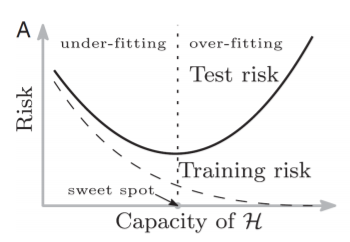
\includegraphics[width=\linewidth]{09/12_27_a}
%     \end{subfigure}
%     \hfill
%     \begin{subfigure}[t]{.5\linewidth}
%         \centering
%         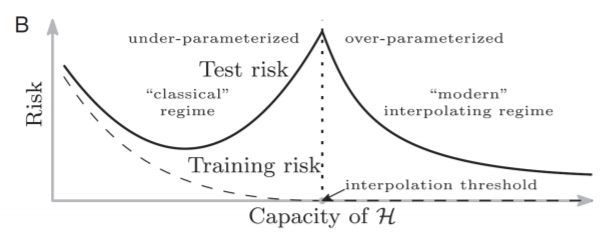
\includegraphics[width=\linewidth]{09/12_27_b}
%     \end{subfigure}
%     \caption{Two plots of the training and validation loss, not as a function of time as before but as a function of \emph{\# network parameters} called \emph{capacity} $\mathcal{H}$.}
%     \label{fig:09:2:double-u-shape}
% \end{figure}


\begin{figure}[H]
    \centering
    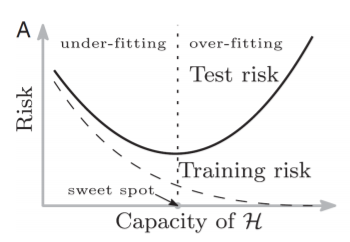
\includegraphics[width=.5\linewidth]{09/12_27_a}
    \caption{Plot of the training and validation loss as a function of model \emph{capacity} $\mathcal{H}$.}
    \label{fig:09:2:capacity-u-shape}
\end{figure}

Looking at \cref{fig:09:2:capacity-u-shape} we recognize the same U-shape seen before (\emph{risk} can be used instead of \emph{error}), but notice the subtle difference: before the plot of the validation error was done as a function of time, while instead this is as a function of \emph{number of network parameters} called \emph{capacity}. The fact that the two plots share similarly shaped curves empirically suggests that the number of parameters and the training time play a similar role on the validation error.

From the plot we can see how the training error is always decreasing as one increases the number of parameters in the network, since the network becomes more and more powerful, meaning it has a larger capacity, i.e. the set
\begin{equation}
    \mathcal{H} = \{ \text{functions that the network can represent well} \}.
\end{equation}
is larger. Eventually, the capacity is so large that there exists a function that perfectly describes the data, so the training error goes to zero. We are overfitting.

The \emph{sweet spot} represents the optimal capacity of the model, meaning it contains a function that describes both the training data and the validation data well enough. 
\\

\textbf{Note.} Early stopping does not directly influence the decision of the  optimal capacity of a model, since it regularizes the training (so we have the training time on the $x$-axis in previous plots).
\\

However, (very) recent results show a somewhat counterintuitive behavior.
\begin{figure}[H]
    \centering
    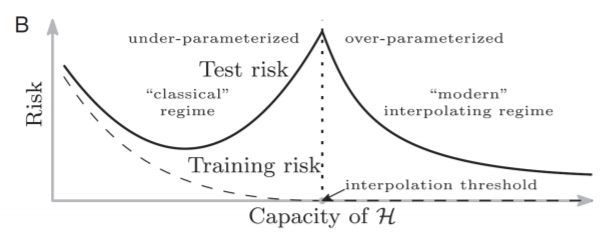
\includegraphics[width=.5\linewidth]{09/12_27_b}
    \caption{Plot of \emph{double descent} curve.}
    \label{fig:09:2:double-u-shape}
\end{figure}

In \cref{fig:09:2:double-u-shape} we see how as one keeps increasing the size of the network, it has been observed that the validation error will eventually start decreasing again, exhibiting what is referred to as \emph{double descent} curve or \emph{double U-shaped} curve.
The point where this happens is called \emph{interpolation threshold}, and it is where we have a perfect fit on the training data (training loss is $0$). 

Although the capacity of $\mathcal{H}$ is already large enough for the training to bring the training error at $0$, further increasing the size of the network and keeping training will not increase the training error, but nonetheless the weights will keep changing a little bit, but also decreasing the validation error. 

This phenomenon has been observed but why it happens is not very clear yet.
One explanation could be that by increasing the number of parameters, such that $\mathcal{H}$ will be a larger set of \emph{function classes} and thus will contain more candidate functions, eventually $\mathcal{H}$ will become so large that one would find a function perfectly compatible with the training data, but that also fits the validation data perfectly.

Quoting the authors of the work that analyzed this behavior:
\begin{center}
    ``By considering \emph{larger function classes}, which contain more candidate predictors compatible with the data, we are able to find interpolating functions that have \emph{smaller norm} and are thus ``\emph{simpler}''. Thus, increasing function class capacity improves the performance of classifiers.''
\end{center}
What they mean by ``interpolating functions that have \emph{smaller norm} and are thus \emph{simpler}'', is that they are basing their assumptions on the \emph{Occam's razor}. If one considers the smoothest (smaller norm) function that fits the data to be the simplest, then by Occam's razor we prefer simpler explanations to the data; however, one may encounter such a function only much later as one increases capacity.

This may seem obvious, since as the capacity of the model goes to infinity, eventually the model can represent any possible function. However, it is indeed surprising that SGD is able to find such good models, producing this double U-shape. As we have said, the training error after the interpolation threshold is nearly $0$, so the gradients driving SGD will not be very informative; nevertheless in all that noise SGD is able, even quite consistently, to find these models.


Different optimization methods from \emph{Stochastic Gradient Descent} (e.g conjugate gradient) yield 
worse generalization because they tend to overfit regions of low non-linearity.\\



\paragraph{Epoch-wise double U-shape}

It has been observed that the double U-shape of the validation loss also appears as a function of training time.

\begin{figure}[H]
    \centering
    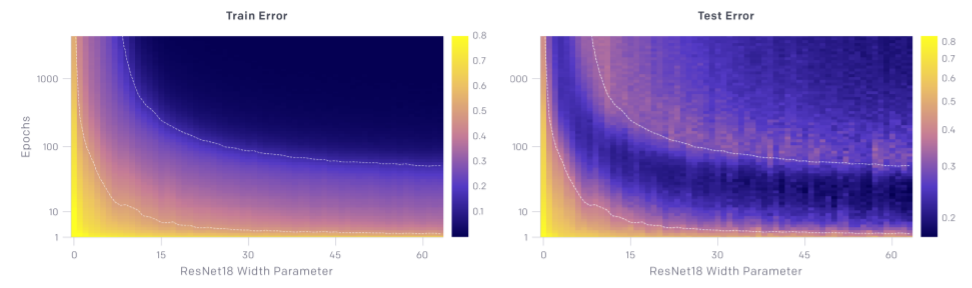
\includegraphics[width=.9\textwidth]{09/14_27}
    \caption{Train error and test error, plotted both against number of parameters and against training time.}
    \label{fig:09:2:double-u-time}
\end{figure}

In \cref{fig:09:2:double-u-time} we can see how for each number of parameters, (taking a ``verical slice'' in the plot) the training error decreases with time (number of epochs). The same can be said if fixing the number of epochs (taking a ``horizontal slice in the plot'') and  considering it as a function of model capacity (width parameter). As we expect, the training error smoothly decreases as a function of both.

On the other hand, it has been observed that the test eror shows the double U-shape not only as a function of model capacity, as we have shown before, but also as a function of training time.
This means that there is a regime where \emph{training longer reverses overfitting}.

\paragraph{How early stopping acts as a regularizer}
So far we have stated that early stopping is a regularization strategy, but we have supported this claim only by showing learning curves where the validation set error has a U-shaped curve. What is the actual mechanism by which early stopping regularizes the model?

\emph{Early stopping} is based on the \emph{smoothness} heuristic:
\begin{center}
    Representational power \emph{grows} with weight magnitude (training time).
\end{center}
This implies the following behavior during training:
\begin{itemize}
    \item Initialize the net with small weights $\vb*{\theta}_0$.
    \item As training time increases, simple hypotheses are considered before complex hypotheses.
    \item Training first explores models similar to what a \emph{a smaller net of optimal size} would have learned.
\end{itemize}

More formally, imagine taking $\tau$ optimization steps (corresponding to $\tau$ training iterations) and with learning rate $\alpha$. We can view the product $\alpha \tau$ as a measure of effective capacity: the model can represent all the functions that can be parametrized by parameters in a sphere of volume proportional to $\alpha \tau$ in the parameter space. 

It has been argued that early stopping has the effect of restricting the optimization procedure to a relatively small volume of parameter space in the neighborhood of the initial parameter value $\vb*{\theta}_0$. Therefore, assuming the gradient is bounded, restricting both the number of iterations $\tau$ and the learning rate $\alpha$ limits the volume of parameter space reachable from $\vb*{\theta}_0$. 

In this sense, $\alpha \tau$ behaves as if it were the reciprocal of the coefficient used for weight decay. Indeed, it can be shown how -- in the case of a simple linear model with a quadratic error function and simple gradient descent -- early stopping is equivalent to $L_2$ regularization.


This heuristic seems to reflect quite well what happens in practice, and thus early stopping is very easy to implement: stop learning when the validation error increases again.